% answers.tex —— 2023 年·全国甲卷·文科 · 参考答案与详细解析片段
% 由 tools/generate_projects.py 依来源总账自 2023/2023_数学真题_全国甲文_试题.md + 2023/2023_数学真题_全国甲文_解析正文.md + 2023/2023_数学真题_全国甲文_答案要点.md 生成，勿手改（改源 MD 后重跑）
\gkpart{2023 年全国甲卷·文科数学 · 试题与答案要点}

\begin{gknotice}
\textbf{解析归属}：下列答案与思路由本库依据固定原卷独立推导，\textbf{不是官方答案}，也不声称代表官方发布版本。

\textbf{证据说明}：全卷 23 题由两名互不知情的求解角色各自独立求解，并逐题进行差异审计。第 1 题的字母差异经原卷选项复核后裁定为 A、集合 $\{2,3,5\}$；第 2—23 题两路结论一致。

\textbf{结构提示}：按本次冻结规格，第 22、23 题\textbf{二选一作答}；为保证内容完整，本文将两题解析均列出。
\end{gknotice}

\gkanswer{答案速查表}

\begin{center}
\begingroup\setlength{\tabcolsep}{4pt}
\begin{tabular}{lllllllllllll}
\toprule
题号 & 1 & 2 & 3 & 4 & 5 & 6 & 7 & 8 & 9 & 10 & 11 & 12 \\
\midrule
答案 & A & C & B & D & C & B & B & C & D & A & A & C \\
\bottomrule
\end{tabular}
\endgroup
\end{center}

\begin{center}
\begin{tabular}{lllll}
\toprule
题号 & 13 & 14 & 15 & 16 \\
\midrule
答案 & $-\dfrac12$ & $2$ & $15$ & $[2\sqrt2,2\sqrt3]$ \\
\bottomrule
\end{tabular}
\end{center}

\par\medskip

\gksubpart{一、单选题}

\begin{answer}
\gksolhead{1}{}

\textbf{题目}：

设全集 $U=\{1,2,3,4,5\}$，集合 $M=\{1,4\}$，$N=\{2,5\}$，则 $N\cup\complement_U M=$（　　）

\begin{gkopts}(4)
\task A．$\{2,3,5\}$
\task B．$\{1,3,4\}$
\task C．$\{1,2,4,5\}$
\task D．$\{2,3,4,5\}$
\end{gkopts}

\textbf{解析}

全集中不属于 $M$ 的元素组成

\[
\complement_U M=\{2,3,5\}.
\]

由于 $N=\{2,5\}\subseteq\complement_U M$，所以

\[
N\cup\complement_U M=\{2,3,5\}.
\]

\gkanswer{答案：A}

\end{answer}
\begin{answer}
\gksolhead{2}{}

\textbf{题目}：

$\dfrac{5(1+\mathrm i^3)}{(2+\mathrm i)(2-\mathrm i)}=$（　　）

\begin{gkopts}(4)
\task A．$-1$
\task B．$1$
\task C．$1-\mathrm i$
\task D．$1+\mathrm i$
\end{gkopts}

\textbf{解析}

由 $\mathrm i^3=-\mathrm i$ 以及

\[
(2+\mathrm i)(2-\mathrm i)=4-\mathrm i^2=5,
\]

可得

\[
\frac{5(1+\mathrm i^3)}{(2+\mathrm i)(2-\mathrm i)}
=\frac{5(1-\mathrm i)}5=1-\mathrm i.
\]

\gkanswer{答案：C}

\end{answer}
\begin{answer}
\gksolhead{3}{}

\textbf{题目}：

已知向量 $\boldsymbol a=(3,1)$，$\boldsymbol b=(2,2)$，则 $\cos\langle\boldsymbol a+\boldsymbol b,\boldsymbol a-\boldsymbol b\rangle=$（　　）

\begin{gkopts}(2)
\task A．$\dfrac1{17}$
\task B．$\dfrac{\sqrt{17}}{17}$
\task C．$\dfrac{\sqrt5}{5}$
\task D．$\dfrac{2\sqrt5}{5}$
\end{gkopts}

\textbf{解析}

先求两向量：

\[
\boldsymbol a+\boldsymbol b=(5,3),\qquad
\boldsymbol a-\boldsymbol b=(1,-1).
\]

因此

\[
\cos\langle\boldsymbol a+\boldsymbol b,\boldsymbol a-\boldsymbol b\rangle
=\frac{5-3}{\sqrt{25+9}\sqrt{1+1}}
=\frac1{\sqrt{17}}=\frac{\sqrt{17}}{17}.
\]

\gkanswer{答案：B}

\end{answer}
\begin{answer}
\gksolhead{4}{}

\textbf{题目}：

某校文艺部有 $4$ 名学生，其中高一、高二年级各 $2$ 名．从这 $4$ 名学生中随机选 $2$ 名组织校文艺汇演，则这 $2$ 名学生来自不同年级的概率为（　　）

\begin{gkopts}(4)
\task A．$\dfrac16$
\task B．$\dfrac13$
\task C．$\dfrac12$
\task D．$\dfrac23$
\end{gkopts}

\textbf{解析}

从 $4$ 人中任取 $2$ 人共有 $\binom42=6$ 种等可能选法。两人来自不同年级时，应从两个年级各选 $1$ 人，共有 $2\times2=4$ 种选法，故所求概率为

\[
\frac46=\frac23.
\]

\gkanswer{答案：D}

\end{answer}
\begin{answer}
\gksolhead{5}{}

\textbf{题目}：

记 $S_n$ 为等差数列 $\{a_n\}$ 的前 $n$ 项和．若 $a_2+a_6=10$，$a_4a_8=45$，则 $S_5=$（　　）

\begin{gkopts}(4)
\task A．$25$
\task B．$22$
\task C．$20$
\task D．$15$
\end{gkopts}

\textbf{解析}

等差数列中，关于 $a_4$ 对称的两项之和为 $2a_4$，所以

\[
a_2+a_6=2a_4=10,
\]

即 $a_4=5$。再由 $a_4a_8=45$ 得 $a_8=9$，从而公差

\[
d=\frac{a_8-a_4}{4}=1.
\]

于是 $a_3=4$，前五项关于 $a_3$ 对称，故

\[
S_5=5a_3=20.
\]

\gkanswer{答案：C}

\end{answer}
\begin{answer}
\gksolhead{6}{}

\textbf{题目}：

执行如图的程序框图，则输出的 $B=$（　　）
\nopagebreak[4]
\begin{center}% 2023 全国甲卷文科 6：程序框图
% 源图流程：输入 n=3,A=1,B=2,k=1；当 k<=n 时依次更新 A、B、k 并折返判断；
% 条件不成立时输出 B。源图所有边均为实线。
\begin{tikzpicture}[font=\small, >=Stealth, node distance=5.5mm, line width=0.4pt,
  box/.style={draw, minimum height=1.9em, minimum width=5.8em, inner xsep=7pt},
  term/.style={draw, rounded corners=7pt, minimum height=1.9em, inner xsep=9pt},
  io/.style={draw, trapezium, trapezium left angle=70, trapezium right angle=110,
             minimum height=1.9em, inner xsep=4pt},
  dec/.style={draw, diamond, aspect=2.6, inner sep=1.5pt}]
  \node[term] (start) {开始};
  \node[io, below=of start] (input) {输入 $n=3,A=1,B=2,k=1$};
  \coordinate[below=3mm of input] (merge);
  \node[dec, below=3mm of merge] (cond) {$k\leqslant n$};
  \node[box, below=of cond] (stepa) {$A=A+B$};
  \node[box, below=of stepa] (stepb) {$B=A+B$};
  \node[box, below=of stepb] (stepk) {$k=k+1$};
  \node[io, below=9mm of stepk] (output) {输出 $B$};
  \node[term, below=of output] (end) {结束};

  % 主流程与“是”分支
  \draw[->] (start) -- (input);
  \draw[->] (input) -- (cond);
  \draw[->] (cond) -- node[right, pos=0.38] {是} (stepa);
  \draw[->] (stepa) -- (stepb);
  \draw[->] (stepb) -- (stepk);

  % k=k+1 后从左侧折返，在输入框与判断框之间重新汇入
  \draw[->] (stepk.west) -- ++(-14mm,0) |- (merge);

  % “否”从菱形右侧绕至输出框上方，再向下进入输出框
  \coordinate[right=16mm of cond] (no-right);
  \coordinate[above=4mm of output] (out-merge);
  \draw (cond.east) -- node[above, pos=0.38] {否} (no-right) |- (out-merge);
  \draw[->] (out-merge) -- (output.north);
  \draw[->] (output) -- (end);
\end{tikzpicture}
\end{center}
\nopagebreak[4]
\begin{gkopts}(4)
\task A．$21$
\task B．$34$
\task C．$55$
\task D．$89$
\end{gkopts}

\textbf{解析}

初始状态为 $(A,B,k)=(1,2,1)$。判断条件成立后，每一轮按顺序更新 $A$、$B$、$k$：

\begin{center}
\begin{tabular}{cccc}
\toprule
轮次 & 更新后的 $A$ & 更新后的 $B$ & 更新后的 $k$ \\
\midrule
1 & $3$ & $5$ & $2$ \\
2 & $8$ & $13$ & $3$ \\
3 & $21$ & $34$ & $4$ \\
\bottomrule
\end{tabular}
\end{center}

第三轮结束后 $k=4>n=3$，程序退出循环并输出 $B=34$。

\gkanswer{答案：B}

\end{answer}
\begin{answer}
\gksolhead{7}{}

\textbf{题目}：

设 $F_1$，$F_2$ 为椭圆 $C:\dfrac{x^2}{5}+y^2=1$ 的两个焦点，点 $P$ 在 $C$ 上，若 $\overrightarrow{PF_1}\cdot\overrightarrow{PF_2}=0$，则 $|PF_1|\cdot|PF_2|=$（　　）

\begin{gkopts}(4)
\task A．$1$
\task B．$2$
\task C．$4$
\task D．$5$
\end{gkopts}

\textbf{解析}

椭圆的长半轴 $a=\sqrt5$，短半轴 $b=1$，故半焦距 $c=2$，从而 $|F_1F_2|=4$。设

\[
x=|PF_1|,\qquad y=|PF_2|.
\]

由椭圆定义，$x+y=2\sqrt5$。向量点积为 $0$ 表明 $PF_1\perp PF_2$，所以

\[
x^2+y^2=|F_1F_2|^2=16.
\]

于是

\[
20=(x+y)^2=x^2+y^2+2xy=16+2xy,
\]

解得 $xy=2$。

\gkanswer{答案：B}

\end{answer}
\begin{answer}
\gksolhead{8}{}

\textbf{题目}：

曲线 $y=\dfrac{\mathrm e^x}{x+1}$ 在点 $\left(1,\dfrac{\mathrm e}{2}\right)$ 处的切线方程为（　　）

\begin{gkopts}(1)
\task A．$y=\dfrac{\mathrm e}{4}x$
\task B．$y=\dfrac{\mathrm e}{2}x$
\task C．$y=\dfrac{\mathrm e}{4}x+\dfrac{\mathrm e}{4}$
\task D．$y=\dfrac{\mathrm e}{2}x+\dfrac{3\mathrm e}{4}$
\end{gkopts}

\textbf{解析}

对函数求导：

\[
y'=\frac{\mathrm e^x(x+1)-\mathrm e^x}{(x+1)^2}
=\frac{x\mathrm e^x}{(x+1)^2}.
\]

在 $x=1$ 处，切线斜率为 $\mathrm e/4$。由点斜式

\[
y-\frac{\mathrm e}{2}=\frac{\mathrm e}{4}(x-1),
\]

整理得

\[
y=\frac{\mathrm e}{4}x+\frac{\mathrm e}{4}.
\]

\gkanswer{答案：C}

\end{answer}
\begin{answer}
\gksolhead{9}{}

\textbf{题目}：

已知双曲线 $C:\dfrac{x^2}{a^2}-\dfrac{y^2}{b^2}=1$（$a>0$，$b>0$）的离心率为 $\sqrt5$，$C$ 的一条渐近线与圆 $(x-2)^2+(y-3)^2=1$ 交于 $A$，$B$ 两点，则 $|AB|=$（　　）

\begin{gkopts}(2)
\task A．$\dfrac{\sqrt5}{5}$
\task B．$\dfrac{2\sqrt5}{5}$
\task C．$\dfrac{3\sqrt5}{5}$
\task D．$\dfrac{4\sqrt5}{5}$
\end{gkopts}

\textbf{解析}

双曲线的离心率满足

\[
\sqrt5=\frac ca=\sqrt{1+\frac{b^2}{a^2}},
\]

故 $b/a=2$，两条渐近线为 $y=\pm2x$。圆心 $(2,3)$ 到直线 $y=2x$ 的距离为

\[
d=\frac{|2\times2-3|}{\sqrt{2^2+(-1)^2}}=\frac1{\sqrt5}<1.
\]

圆心到另一条渐近线 $y=-2x$ 的距离为 $7/\sqrt5>1$，所以只有 $y=2x$ 截得弦 $AB$。由弦长公式，

\[
|AB|=2\sqrt{1-d^2}
=2\sqrt{1-\frac15}
=\frac{4\sqrt5}{5}.
\]

\gkanswer{答案：D}

\end{answer}
\begin{answer}
\gksolhead{10}{}

\textbf{题目}：

在三棱锥 $P-ABC$ 中，$\triangle ABC$ 是边长为 $2$ 的等边三角形，$PA=PB=2$，$PC=\sqrt6$，则该棱锥的体积为（　　）

\begin{gkopts}(4)
\task A．$1$
\task B．$\sqrt3$
\task C．$2$
\task D．$3$
\end{gkopts}

\textbf{解析}

在平面 $z=0$ 内取

\[
A=(-1,0,0),\quad B=(1,0,0),\quad C=(0,\sqrt3,0).
\]

由 $PA=PB$，可设 $P=(0,y,h)$。条件 $PA=2$ 给出

\[
1+y^2+h^2=4,
\]

即 $y^2+h^2=3$。又由 $PC=\sqrt6$，

\[
(y-\sqrt3)^2+h^2=6.
\]

两式相减得 $y=0$，继而 $h=\sqrt3$。底面等边三角形面积为 $\sqrt3$，所以棱锥体积为

\[
V=\frac13\cdot\sqrt3\cdot\sqrt3=1.
\]

\gkanswer{答案：A}

\end{answer}
\begin{answer}
\gksolhead{11}{}

\textbf{题目}：

已知函数 $f(x)=\mathrm e^{-(x-1)^2}$．记 $a=f\left(\dfrac{\sqrt2}{2}\right)$，$b=f\left(\dfrac{\sqrt3}{2}\right)$，$c=f\left(\dfrac{\sqrt6}{2}\right)$，则（　　）

\begin{gkopts}(4)
\task A．$b>c>a$
\task B．$b>a>c$
\task C．$c>b>a$
\task D．$c>a>b$
\end{gkopts}

\textbf{解析}

函数 $f(x)=\mathrm e^{-(x-1)^2}$ 的值只由 $|x-1|$ 决定，并随该距离增大而减小。三个自变量到 $1$ 的距离满足

\[
1-\frac{\sqrt3}{2}
<\frac{\sqrt6}{2}-1
<1-\frac{\sqrt2}{2}.
\]

因此相应函数值的大小关系为

\[
b>c>a.
\]

\gkanswer{答案：A}

\end{answer}
\begin{answer}
\gksolhead{12}{}

\textbf{题目}：

函数 $y=f(x)$ 的图象由函数 $y=\cos\left(2x+\dfrac\pi6\right)$ 的图象向左平移 $\dfrac\pi6$ 个单位长度得到，则 $y=f(x)$ 的图象与直线 $y=\dfrac12x-\dfrac12$ 的交点个数为（　　）

\begin{gkopts}(4)
\task A．$1$
\task B．$2$
\task C．$3$
\task D．$4$
\end{gkopts}

\textbf{解析}

原函数图象向左平移 $\pi/6$ 后，

\[
f(x)=\cos\left(2\left(x+\frac\pi6\right)+\frac\pi6\right)
=\cos\left(2x+\frac\pi2\right)=-\sin2x.
\]

令

\[
H(x)=-\sin2x-\frac x2+\frac12.
\]

交点横坐标就是 $H(x)=0$ 的根。由于 $-\sin2x\in[-1,1]$，有根时必有 $x/2-1/2\in[-1,1]$，即 $x\in[-1,3]$。当 $x\in[-1,0]$ 时，$2x\in[-2,0]\subset(-\pi,0]$，故 $-\sin2x\geqslant0$，且 $-x/2+1/2>0$，所以该段无根。

设

\[
\beta=\frac12\arccos\left(-\frac14\right).
\]

由

\[
H'(x)=-2\cos2x-\frac12
\]

可知，在 $(0,3)$ 内只有两个驻点 $\beta$、$\pi-\beta$，并且 $H$ 在

\[
(0,\beta),\quad(\beta,\pi-\beta),\quad(\pi-\beta,3)
\]

上依次单调递减、单调递增、单调递减。下面给出不依赖数值扫描的符号判定：

\[
H(0)=\frac12>0,
\]

而 $\sin(2\beta)=\sqrt{15}/4$，故

\[
H(\beta)=\frac12-\frac{\sqrt{15}}4-\frac\beta2<0.
\]

又因 $\arccos(-1/4)<2\pi/3$，所以 $\beta<\pi/3$，从而

\[
\beta<2<\pi-\beta.
\]

并且 $7\pi/6<4<3\pi/2$，故 $\sin4<-1/2$，于是

\[
H(2)=-\sin4-\frac12>0.
\]

最后，$3\pi/2<6<2\pi$，故 $-1<\sin6<0$，从而

\[
H(3)=-\sin6-1<0.
\]

因此，三个单调区间上分别恰有一个根，而 $[-1,0]$ 上没有根。交点个数恰为 $3$。

\gkanswer{答案：C}

\par\medskip

\gksubpart{二、填空题}

\end{answer}
\begin{answer}
\gksolhead{13}{}

\textbf{题目}：

记 $S_n$ 为等比数列 $\{a_n\}$ 的前 $n$ 项和．若 $8S_6=7S_3$，则 $\{a_n\}$ 的公比为 \gkblank{}．

\textbf{解析}

设公比为 $q$。由等比数列分段求和，

\[
S_6=S_3+q^3S_3=S_3(1+q^3).
\]

又 $S_3=a_1(1+q+q^2)\ne0$，因为 $a_1\ne0$，且实数范围内 $1+q+q^2>0$。代入 $8S_6=7S_3$，得

\[
8(1+q^3)=7,
\]

所以

\[
q^3=-\frac18,\qquad q=-\frac12.
\]

\gkanswer{答案：$-\dfrac12$}

\end{answer}
\begin{answer}
\gksolhead{14}{}

\textbf{题目}：

若 $f(x)=(x-1)^2+ax+\sin\left(x+\dfrac\pi2\right)$ 为偶函数，则 $a=$ \gkblank{}．

\textbf{解析}

利用 $\sin(x+\pi/2)=\cos x$，可将函数写成

\[
f(x)=x^2+(a-2)x+1+\cos x.
\]

其中 $x^2$、常数项和 $\cos x$ 均为偶函数，因此一次项必须消失，即

\[
a-2=0.
\]

故 $a=2$。

\gkanswer{答案：$2$}

\end{answer}
\begin{answer}
\gksolhead{15}{}

\textbf{题目}：

若 $x$，$y$ 满足约束条件 $\begin{cases}3x-2y\leqslant3,\\-2x+3y\leqslant3,\\x+y\geqslant1,\end{cases}$ 则 $z=3x+2y$ 的最大值为 \gkblank{}．

\textbf{解析}

三条边界线两两相交，且满足全部约束的顶点为

\[
(1,0),\qquad(0,1),\qquad(3,3).
\]

线性目标函数 $z=3x+2y$ 在三个顶点的值依次为

\[
3,\qquad2,\qquad15.
\]

所以最大值为 $15$。

\gkanswer{答案：$15$}

\end{answer}
\begin{answer}
\gksolhead{16}{}

\textbf{题目}：

在正方体 $ABCD-A_1B_1C_1D_1$ 中，$AB=4$，$O$ 为 $AC_1$ 的中点．若该正方体的棱与球 $O$ 的球面有公共点，则球 $O$ 的半径的取值范围是 \gkblank{}．

\textbf{解析}

$AC_1$ 是正方体的体对角线，故其中点 $O$ 是正方体中心。取任意一条棱，并以棱中点为参数原点；棱上点到 $O$ 的距离在棱中点处最小，在两个端点处最大。

中心到棱中点的距离为半个面对角线，即 $2\sqrt2$；中心到端点的距离为半个体对角线，即 $2\sqrt3$。距离沿棱连续变化，所以球面与正方体的棱有公共点当且仅当

\[
2\sqrt2\leqslant r\leqslant2\sqrt3.
\]

\gkanswer{答案：$[2\sqrt2,2\sqrt3]$}

\par\medskip

\gksubpart{三、解答题}

\end{answer}
\begin{answer}
\gksolhead{17}{}

\textbf{题目}：

记 $\triangle ABC$ 的内角 $A$，$B$，$C$ 的对边分别为 $a$，$b$，$c$，已知 $\dfrac{b^2+c^2-a^2}{\cos A}=2$．

  (1) 求 $bc$；

  (2) 若 $\dfrac{a\cos B-b\cos A}{a\cos B+b\cos A}-\dfrac bc=1$，求 $\triangle ABC$ 的面积．

\textbf{解析}

\gksubpart{(1)}

由余弦定理，

\[
b^2+c^2-a^2=2bc\cos A.
\]

题设分式有意义，故 $\cos A\ne0$。代入已知条件，得

\[
2bc=2,
\]

所以 $bc=1$。

\gksubpart{(2)}

由余弦定理，

\[
a\cos B=\frac{a^2+c^2-b^2}{2c},\qquad
b\cos A=\frac{b^2+c^2-a^2}{2c}.
\]

因此

\[
a\cos B-b\cos A=\frac{a^2-b^2}{c},\qquad
a\cos B+b\cos A=c.
\]

原条件化为

\[
\frac{a^2-b^2}{c^2}-\frac bc=1,
\]

即

\[
a^2-b^2=c^2+bc.
\]

另一方面，余弦定理给出

\[
a^2-b^2=c^2-2bc\cos A.
\]

比较两式，并利用 $bc=1$，得 $\cos A=-1/2$，所以 $A=2\pi/3$。三角形面积为

\[
S=\frac12bc\sin A
=\frac12\cdot1\cdot\frac{\sqrt3}{2}
=\frac{\sqrt3}{4}.
\]

\gkanswer{答案（1）：$bc=1$}

\gkanswer{答案（2）：$\dfrac{\sqrt3}{4}$}

\end{answer}
\begin{answer}
\gksolhead{18}{}

\textbf{题目}：

如图，在三棱柱 $ABC-A_1B_1C_1$ 中，$A_1C\perp$ 平面 $ABC$，$\angle ACB=90^\circ$．
\nopagebreak[4]
\begin{center}% 2023 全国甲卷文科 18：三棱柱 ABC-A1B1C1
% 源图点位与遮挡：底面 AC、CB 及棱 CC1 被遮挡；题设线段 A1C 也画为虚线。
% 可见棱和题设线段 A1B 为实线。源图没有直角、长度或等长标记。
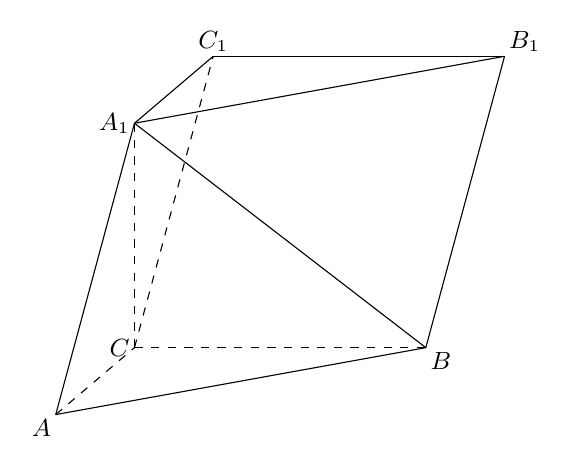
\begin{tikzpicture}[font=\small, line width=0.4pt,
  every node/.style={inner sep=1.5pt}]
  % 图纸坐标只用于复现原卷投影；上下两个三角形保持同一平移向量。
  \coordinate (A)  at (0,0);
  \coordinate (C)  at (1.00,0.85);
  \coordinate (B)  at (4.70,0.85);
  \coordinate (A1) at (1.00,3.70);
  \coordinate (C1) at (2.00,4.55);
  \coordinate (B1) at (5.70,4.55);

  % 遮挡棱及题设虚线先画，保证交叉处的可见实线在前。
  \draw[dashed] (A) -- (C);
  \draw[dashed] (C) -- (B);
  \draw[dashed] (C) -- (C1);
  \draw[dashed] (A1) -- (C);

  % 可见棱
  \draw (A) -- (B);
  \draw (A) -- (A1);
  \draw (A1) -- (C1);
  \draw (C1) -- (B1);
  \draw (B1) -- (B);
  \draw (A1) -- (B1);

  % 题面明确画出的线段 A1B
  \draw (A1) -- (B);

  % 顶点标注
  \node[anchor=north east] at (A)  {$A$};
  \node[anchor=east]       at (C)  {$C$};
  \node[anchor=north west] at (B)  {$B$};
  \node[anchor=east]       at (A1) {$A_1$};
  \node[anchor=south]      at (C1) {$C_1$};
  \node[anchor=south west] at (B1) {$B_1$};
\end{tikzpicture}
\end{center}
\nopagebreak[4]
  (1) 证明：平面 $ACC_1A_1\perp$ 平面 $BB_1C_1C$；

  (2) 设 $AB=A_1B$，$AA_1=2$，求四棱锥 $A_1-BB_1C_1C$ 的高．

\textbf{解析}

\gksubpart{(1)}

由 $A_1C\perp$ 平面 $ABC$，得 $A_1C\perp BC$。又 $\angle ACB=90^\circ$，所以 $AC\perp BC$。线段 $AC$、$A_1C$ 是平面 $ACC_1A_1$ 内相交于 $C$ 的两条直线，故

\[
BC\perp\text{\text{平面} }ACC_1A_1.
\]

由于 $BC\subset\text{\text{平面} }BB_1C_1C$，可知

\[
\text{\text{平面} }ACC_1A_1\perp\text{\text{平面} }BB_1C_1C.
\]

\gksubpart{(2)}

设 $AC=x$，$A_1C=h$。因为 $AC\perp BC$ 且 $A_1C\perp BC$，

\[
AB^2=x^2+BC^2,
\qquad
A_1B^2=h^2+BC^2.
\]

由 $AB=A_1B$ 得 $x=h$。在直角三角形 $ACA_1$ 中，

\[
AA_1^2=AC^2+A_1C^2=x^2+h^2=4,
\]

故 $x=h=\sqrt2$。

取

\[
C=(0,0,0),\quad A=(x,0,0),\quad B=(0,b,0),\quad A_1=(0,0,h).
\]

三棱柱的平移向量为 $\overrightarrow{AA_1}=(-x,0,h)$，所以平面 $BB_1C_1C$ 由方向向量 $(0,b,0)$ 与 $(-x,0,h)$ 张成，其法向量可取 $(h,0,x)$。点 $A_1$ 到该平面的距离为

\[
d=\frac{|(h,0,x)\cdot(0,0,h)|}{\sqrt{h^2+x^2}}
=\frac{xh}{\sqrt{x^2+h^2}}
=\frac2{2}=1.
\]

这就是四棱锥 $A_1-BB_1C_1C$ 的高。

\gkanswer{答案（1）：见解析版}

\gkanswer{答案（2）：$1$}

\end{answer}
\begin{answer}
\gksolhead{19}{}

\textbf{题目}：

一项试验旨在研究臭氧效应，试验方案如下：选 $40$ 只小白鼠，随机地将其中 $20$ 只分配到试验组，另外 $20$ 只分配到对照组，试验组的小白鼠饲养在高浓度臭氧环境，对照组的小白鼠饲养在正常环境，一段时间后统计每只小白鼠体重的增加量（单位：g）．试验结果如下：

对照组的小白鼠体重的增加量从小到大排序为

$15.2\quad18.8\quad20.2\quad21.3\quad22.5\quad23.2\quad25.8\quad26.5\quad27.5\quad30.1$

$32.6\quad34.3\quad34.8\quad35.6\quad35.6\quad35.8\quad36.2\quad37.3\quad40.5\quad43.2$

试验组的小白鼠体重的增加量从小到大排序为

$7.8\quad9.2\quad11.4\quad12.4\quad13.2\quad15.5\quad16.5\quad18.0\quad18.8\quad19.2$

$19.8\quad20.2\quad21.6\quad22.8\quad23.6\quad23.9\quad25.1\quad28.2\quad32.3\quad36.5$

  (1) 计算试验组的样本平均数；

  (2) ① 求 $40$ 只小白鼠体重的增加量的中位数 $m$，再分别统计两样本中小于 $m$ 与不小于 $m$ 的数据的个数，完成如下列联表：

\begin{center}
\begin{tabular}{ccc}
\toprule
 & $<m$ & $\geqslant m$ \\
\midrule
对照组 &  &  \\
试验组 &  &  \\
\bottomrule
\end{tabular}
\end{center}

　　② 根据①中的列联表，能否有 $95\%$ 的把握认为小白鼠在高浓度臭氧环境中与在正常环境中体重的增加量有差异？

附：$K^2=\dfrac{n(ad-bc)^2}{(a+b)(c+d)(a+c)(b+d)}$，

\begin{center}
\begin{tabular}{cccc}
\toprule
$P(K^2\geqslant k)$ & $0.100$ & $0.050$ & $0.010$ \\
\midrule
$k$ & $2.706$ & $3.841$ & $6.635$ \\
\bottomrule
\end{tabular}
\end{center}

\textbf{解析}

\gksubpart{(1)}

试验组 $20$ 个数据之和为

\[
7.8+9.2+\cdots+32.3+36.5=396.0.
\]

因此样本平均数为

\[
\bar x=\frac{396.0}{20}=19.8\,\mathrm g.
\]

\gksubpart{(2)}

\textbf{① 中位数与列联表}

合并两组数据并从小到大排列，第 $20$、$21$ 个数据分别为 $23.2$、$23.6$，所以

\[
m=\frac{23.2+23.6}{2}=23.4.
\]

逐项计数得到

\begin{center}
\begin{tabular}{ccc}
\toprule
 & $<m$ & $\geqslant m$ \\
\midrule
对照组 & $6$ & $14$ \\
试验组 & $14$ & $6$ \\
\bottomrule
\end{tabular}
\end{center}

\textbf{② 独立性检验}

按题给公式取 $n=40$，$a=6$，$b=14$，$c=14$，$d=6$，则

\[
K^2
=\frac{40(6\times6-14\times14)^2}{20\times20\times20\times20}
=\frac{40\times160^2}{20^4}
=6.4.
\]

由于

\[
6.4>3.841,
\]

所以按题设检验口径，有 $95\%$ 的把握认为小白鼠在高浓度臭氧环境中与在正常环境中体重的增加量有差异。

\gkanswer{答案（1）：$19.8\,\mathrm g$}

\gkanswer{答案（2）：$m=23.4$；列联表中对照组为 $(6,14)$、试验组为 $(14,6)$；$K^2=6.4$，有 $95\%$ 的把握认为体重增加量有差异}

\end{answer}
\begin{answer}
\gksolhead{20}{}

\textbf{题目}：

已知函数 $f(x)=ax-\dfrac{\sin x}{\cos^2x}$，$x\in\left(0,\dfrac\pi2\right)$．

  (1) 当 $a=1$ 时，讨论 $f(x)$ 的单调性；

  (2) 若 $f(x)+\sin x<0$，求 $a$ 的取值范围．

\textbf{解析}

\gksubpart{(1)}

当 $a=1$ 时，

\[
f'(x)=1-\left(\frac{\sin x}{\cos^2x}\right)'
=1-\frac{1+\sin^2x}{\cos^3x}.
\]

在 $0<x<\pi/2$ 上，有 $0<\cos x<1$，故

\[
1+\sin^2x>1>\cos^3x.
\]

于是 $f'(x)<0$，所以 $f$ 在 $\left(0,\pi/2\right)$ 上单调递减。

\gksubpart{(2)}

按题意，不等式应对定义域中的每个 $x$ 成立。将其化简：

\[
f(x)+\sin x
=ax-\frac{\sin x}{\cos^2x}+\sin x
=ax-\frac{\sin^3x}{\cos^2x}<0.
\]

因为 $x>0$，这等价于

\[
a<g(x):=\frac{\sin^3x}{x\cos^2x}
\]

对一切 $x\in(0,\pi/2)$ 成立。该区间内 $g(x)>0$，并且

\[
\lim_{x\to0^+}g(x)=0.
\]

所以 $g$ 的下确界为 $0$，且不取到。当 $a\leqslant0$ 时，不等式对每个 $x$ 都严格成立；当 $a>0$ 时，由上述极限可取充分小的 $x$ 使 $g(x)<a$，条件不成立。因此

\[
a\leqslant0.
\]

\gkanswer{答案（1）：在 $\left(0,\dfrac\pi2\right)$ 上单调递减}

\gkanswer{答案（2）：$a\leqslant0$}

\end{answer}
\begin{answer}
\gksolhead{21}{}

\textbf{题目}：

已知直线 $x-2y+1=0$ 与抛物线 $C:y^2=2px$（$p>0$）交于 $A$，$B$ 两点，$|AB|=4\sqrt{15}$．

  (1) 求 $p$；

  (2) 设 $F$ 为 $C$ 的焦点，$M$，$N$ 为 $C$ 上两点，且 $\overrightarrow{FM}\cdot\overrightarrow{FN}=0$，求 $\triangle MFN$ 面积的最小值．

\textbf{解析}

\gksubpart{(1)}

由直线方程得 $x=2y-1$。代入抛物线方程，得到关于交点纵坐标的方程

\[
y^2-4py+2p=0.
\]

设两根为 $y_1$、$y_2$，则

\[
(y_1-y_2)^2=16p^2-8p.
\]

直线上两点满足 $\Delta x=2\Delta y$，所以

\[
|AB|^2=5(y_1-y_2)^2=5(16p^2-8p).
\]

由 $|AB|=4\sqrt{15}$，得

\[
5(16p^2-8p)=240,
\]

即 $2p^2-p-6=0$。结合 $p>0$，可得 $p=2$。

\gksubpart{(2)}

此时抛物线为 $y^2=4x$，焦点为 $F=(1,0)$，准线为 $x=-1$。从焦点出发、方向角为 $\theta$ 的射线与抛物线交于一点，设焦半径为 $r$。由抛物线定义，

\[
r=x+1=2+r\cos\theta,
\]

故

\[
r=\frac2{1-\cos\theta}.
\]

两条焦半径互相垂直。交换 $M$、$N$ 并在必要时将 $\theta$ 换成 $-\theta$，可令它们的方向角为 $\theta$ 与 $\theta+\pi/2$。于是

\[
FM=\frac2{1-\cos\theta},\qquad
FN=\frac2{1+\sin\theta}.
\]

三角形 $MFN$ 在 $F$ 处为直角，因此面积

\[
S=\frac12FM\cdot FN
=\frac2{(1-\cos\theta)(1+\sin\theta)}.
\]

下面直接在共同约束下求分母的全局最大值。令

\[
u=-\cos\theta,\qquad v=\sin\theta,\qquad s=u+v.
\]

则 $u^2+v^2=1$，且 $-\sqrt2\leqslant s\leqslant\sqrt2$。由

\[
uv=\frac{s^2-1}{2}
\]

可得

\[
(1+u)(1+v)
=1+s+uv
=\frac{(s+1)^2}{2}
\leqslant\frac{(1+\sqrt2)^2}{2}
=\frac{3+2\sqrt2}{2}.
\]

等号在 $u=v=1/\sqrt2$，即 $\theta=3\pi/4$ 时取得，对应两点均为抛物线上的有限点。因此

\[
S_{\min}
=\frac{2}{(3+2\sqrt2)/2}
=\frac4{3+2\sqrt2}
=12-8\sqrt2.
\]

\gkanswer{答案（1）：$p=2$}

\gkanswer{答案（2）：$12-8\sqrt2$}

\gksubpart{选考题（第 22、23 题二选一）}

\end{answer}
\begin{answer}
\gksolhead{22}{}

\textbf{题目}：

已知点 $P(2,1)$，直线 $l:\begin{cases}x=2+t\cos\alpha,\\y=1+t\sin\alpha\end{cases}$（$t$ 为参数），$\alpha$ 为 $l$ 的倾斜角，$l$ 与 $x$ 轴正半轴、$y$ 轴正半轴分别交于点 $A$，$B$，且 $|PA|\cdot|PB|=4$．

  (1) 求 $\alpha$；

  (2) 以坐标原点为极点，$x$ 轴正半轴为极轴建立极坐标系，求 $l$ 的极坐标方程．

\textbf{解析}

\gksubpart{(1)}

直线过 $P(2,1)$，方向向量为 $(\cos\alpha,\sin\alpha)$。由于它与两坐标轴的正半轴均相交，斜率为负，故

\[
\frac\pi2<\alpha<\pi.
\]

与 $x$ 轴交于 $A$ 时，参数满足

\[
1+t_A\sin\alpha=0,
\]

所以 $|PA|=|t_A|=1/\sin\alpha$。与 $y$ 轴交于 $B$ 时，

\[
2+t_B\cos\alpha=0,
\]

所以 $|PB|=|t_B|=-2/\cos\alpha$。由距离之积为 $4$，得

\[
-\frac2{\sin\alpha\cos\alpha}=4,
\]

即 $\sin\alpha\cos\alpha=-1/2$。结合倾斜角范围，

\[
\alpha=\frac{3\pi}{4}.
\]

\gksubpart{(2)}

直线斜率为 $-1$，且过 $(2,1)$，故直角坐标方程为

\[
x+y=3.
\]

代入 $x=\rho\cos\theta$、$y=\rho\sin\theta$，得到极坐标方程

\[
\rho(\cos\theta+\sin\theta)=3.
\]

\gkanswer{答案（1）：$\alpha=\dfrac{3\pi}{4}$}

\gkanswer{答案（2）：$\rho(\cos\theta+\sin\theta)=3$}

\end{answer}
\begin{answer}
\gksolhead{23}{}

\textbf{题目}：

设 $a>0$，函数 $f(x)=2|x-a|-a$．

  (1) 求不等式 $f(x)<x$ 的解集；

  (2) 若曲线 $y=f(x)$ 与 $x$ 轴所围成的图形的面积为 $2$，求 $a$．

\textbf{解析}

\gksubpart{(1)}

当 $x<a$ 时，

\[
f(x)=2(a-x)-a=a-2x.
\]

由 $a-2x<x$ 得 $x>a/3$，结合 $x<a$，得到 $a/3<x<a$。

当 $x\geqslant a$ 时，

\[
f(x)=2(x-a)-a=2x-3a.
\]

由 $2x-3a<x$ 得 $x<3a$，结合 $x\geqslant a$，得到 $a\leqslant x<3a$。两段合并，不等式的解集为

\[
\left(\frac a3,3a\right).
\]

\gksubpart{(2)}

函数图象的顶点为 $(a,-a)$。令 $f(x)=0$，得到两个零点

\[
x=\frac a2,\qquad x=\frac{3a}{2}.
\]

曲线与 $x$ 轴所围图形是底长、高均为 $a$ 的三角形，面积为 $a^2/2$。由

\[
\frac12a^2=2
\]

及 $a>0$，可得 $a=2$。

\gkanswer{答案（1）：$\left(\dfrac a3,3a\right)$}

\gkanswer{答案（2）：$a=2$}

\end{answer}